%!TEX root = ../concur2021.tex

%\subsection{Proofs for section 5 } \label{sec:app-relations}

%\begin{theorem}\label{theorem:strong_equal_weak_p2p}
%	A peer-to-peer MSC is \skSous{k} iff it is weakly-$k$-synchronous.
%\end{theorem}

\subsection{Proofs}
\label{app:stronglykp2p}
%\strongequalweakptop*
%
Proof of the property from Remark~\ref{rem:stronglykp2p}:
\begin{restatable}{proposition}{strongequalweakptop}
\label{proposition:strong_equal_weak_p2p}
%	A \pp MSC is \skSo{k} iff it is \wkSo{k}.
Consider an MSC of the form
$\msc = \msc_1 \cdot \ldots \cdot \msc_n$ %(with $\msc_i$ an MSC)
such that every MSC $\msc_i = (\Events_i,\procrel_i,\lhd_i,\lambda_i)$ is a ($k$-)exchange.
Then, for all $(e,f) \in {\le}_\msc$, there are $1 \le i \le j \le n$
such that $e \in \Events_i$ and $f \in \Events_j$.
\end{restatable}

\begin{proof}
%	$\Rightarrow$ By definition.
%%\alain{I change the direction of implications}
%
%	$\Leftarrow$ Let $\msc \in \MSCs$ such that $\msc$ is \wkSo{k}.
%	By contradiction, suppose that $\msc$ is not \skSo{k}. Then:
%	\begin{itemize}
%		\item either there is no decomposition such that $M = M_1 \cdots M_n$, $M_i$ is a \kE{k}, $1 \le i \le n$, and so $M$ cannot be \wkSo{k}, which is a contradition;
%		\item or there is $e \le_M f $ such that $e \in \Events_i, f \in \Events_j$, $i>j$. If $ e \le_M f$, either $e \lhd f$ and so $i = j$, or there is $ p \in \procSet$ such that $e \rightarrow_p f$ and $e$ appears always before $f$ on $p$ thus $i \le j$, and so we have a contradiction. \qedhere
%	\end{itemize}
%	%\qed
If $e \le_\msc f$, then there is a sequence of events $e = e_0 \bowtie_1 e_1 \bowtie_2 \ldots
\bowtie_m e_m = f$ where $\bowtie$ is either $\to$ or $\lhd$. Clearly, for every
$\ell \in \{0,\ldots,m-1\}$, there are $1 \le i \le j \le n$
such that $e_\ell \in \Events_i$ and $e_{\ell+1} \in \Events_j$.
By transitivity, this proves the statement.
\qedhere
	%\qed
\end{proof}




\synchroinexists*
\begin{proof}
We begin by considering a \pp MSC.
	Let $\msc \in \MSCs$ be such that $M$ is \skSo{k}. Then, there is $M = M_1 \cdots M_n$, $M_i$ which is a \kE{k}, $1 \le i \le n$.
	By induction on $\msc$:
	\begin{itemize}
		\item[\textbf{1.}]\textbf{Base} $\msc = \msc_1$ then $\msc$ is a \kE{k} and by definition $|\Matched{\msc} \cup \Unm{\msc}| \leq k$.
		Then,  for all $e \in Matched(M)$ s.t. $\lambda(e) = \sact{p}{q}{\msg}$, we have
		\[\sametype{e}{\pqsAct{p}{q}}{\linrel} - \sametype{e}{\pqrAct{p}{q}}{\linrel} \le k.\]
		Then, $M$ is $k$-p2p-bounded.
		\item[\textbf{2.}]\textbf{Step}
		$M = M' \cdot M_n$ and we suppose that $M' = M_1 \cdots M_{n-1}$ is $k$-p2p-bounded.
		For all $1\leq i\leq {n}$, $M_i$ is a \kE{k}, and so an MSC, and by definition we know that any reception belongs to the same MSC as its matched send.
		Let $\lin$ be a linearization and $f \in Matched(M')$ s.t. $\lambda(f) = \sact{p}{q}{\msg}$ and, for all $e \in Matched(M')$ s.t. $\lambda(e) = \sact{p}{q}{\msg}$,  \[\sametype{f}{\pqsAct{p}{q}}{\linrel} > \sametype{e}{\pqsAct{p}{q}}{\linrel}.\]
		Then, we have:
		\[\sametype{f}{\pqsAct{p}{q}}{\linrel} - \sametype{f}{\pqrAct{p}{q}}{\linrel} = 0.\]
		Note that there is no unmatched message sent to $q$ before $f$ as $f$ is matched.
		As $M_n$ is a \kE{k}, we have for all  $e \in Matched(M_n)$ s.t. $\lambda(e) = \sact{p}{q}{\msg}$
		\[\sametype{e}{\pqsAct{p}{q}}{\linrel} - \sametype{e}{\pqrAct{p}{q}}{\linrel} \le k.\]

		Finally, for all  $e' \in Matched(M)$ s.t. $\lambda(e') = \sact{p}{q}{\msg}$, there is $e \in Matched(M_n)$ such that we can decompose:
		\[\sametype{e'}{\pqsAct{p}{q}}{\linrel} = \sametype{f}{\pqsAct{p}{q}}{\linrel} + \sametype{e}{\pqsAct{p}{q}}{\linrel} \]
		and
		\[\sametype{e'}{\pqrAct{p}{q}}{\linrel} =  \sametype{f}{\pqrAct{p}{q}}{\linrel} + \sametype{e}{\pqrAct{p}{q}}{\linrel}.\]
		Therefore \[ \sametype{e'}{\pqsAct{p}{q}}{\linrel} - \sametype{e'}{\pqrAct{p}{q}}{\linrel} \le k.\]
		Then, $M$ is $k$-p2p-bounded.
	\end{itemize}

Now, we move to  mailbox MSCs.
		Let $M \in \mbMSCs$ be a \skSo{k} MSC.
	By definition, $M = M_1 \cdots M_n$ such that every $M_i=(\Events_i,\procrel_i,\lhd_i,\lambda_i)$ is a \kE{k} and, for all $(e,f) \in {\sqsubset}_\msc$, there are indices $1 \leq i < j \leq n$ such that $e \in \Events_i$ and $f \in \Events_j$.

	By induction of $M$, we show that $M$ is $k$-mailbox-bounded.
	\begin{itemize}
		\item[\textbf{1.}]\textbf{Base}
		$M = M_1$ then $M$ is a \kE{k} and $|\Matched{\msc} \cup \Unm{\msc}| \le k$. Let $\lin$ be any linearization of $M$ and so, for all $e \in Matched(M)$ s.t. $\lambda(e) = \sact{p}{q}{\msg}$, we have
		$\sametype{e}{\pqsAct{\plh}{q}}{\linrel} - \sametype{e}{\pqrAct{\plh}{q}}{\linrel} \le k$. Then, $M$ is $k$-mailbox-bounded.
		\item[\textbf{2.}]\textbf{Step}
 $M = M' \cdot M_n$ and we suppose that $M' = M_1 \cdots M_{n-1}$ is $k$-mailbox-bounded.
		For all $1\leq i\leq {n}$, $M_i$ is a \kE{k}, and so an MSC, and by definition we know that any reception belongs to the same MSC as its matched send.
		Let $\lin$ be a linearization and $f \in Matched(M')$ s.t. $\lambda(f) = \sact{p}{q}{\msg}$ and, for all $e \in Matched(M')$ s.t. $\lambda(e) = \sact{p}{q}{\msg}$,
		\[\sametype{f}{\pqsAct{\plh}{q}}{\linrel} > \sametype{e}{\pqsAct{\plh}{q}}{\linrel}.\]
		Then, we have:
		\[\sametype{f}{\pqsAct{\plh}{q}}{\linrel} - \sametype{f}{\pqrAct{\plh}{q}}{\linrel} = 0.\]
		Note that there is no unmatched message sent to $q$ before $f$ as $f$ is matched.
		As $M_n$ is a \kE{k}, we have for all  $e \in Matched(M_n)$ s.t. $\lambda(e) = \sact{p}{q}{\msg}$
		\[\sametype{e}{\pqsAct{\plh}{q}}{\linrel} - \sametype{e}{\pqrAct{\plh}{q}}{\linrel} \le k.\]
		Finally, for all  $e' \in Matched(M)$ s.t. $\lambda(e') = \sact{p}{q}{\msg}$, there is $e \in Matched(M_n)$ such that we can decompose:
		\[\sametype{e'}{\pqsAct{\plh}{q}}{\linrel} = \sametype{f}{\pqsAct{\plh}{q}}{\linrel} + \sametype{e}{\pqsAct{\plh}{q}}{\linrel} \]
		and
		\[\sametype{e'}{\pqrAct{\plh}{q}}{\linrel} =  \sametype{f}{\pqrAct{\plh}{q}}{\linrel} + \sametype{e}{\pqrAct{\plh}{q}}{\linrel}.\]
		Therefore \[  \sametype{e'}{\pqsAct{\plh}{q}}{\linrel} - \sametype{e'}{\pqrAct{\plh}{q}}{\linrel} \le k.\]
		Then, $M$ is $k$-mailbox-bounded.
	\end{itemize}%\qed
\end{proof}


\weakuniveruweak*

\begin{proof}

	Let $\System$ be a system such that, for all $\msc \in \MSCs$, $\msc = \msc_1 \cdots \msc_n$ where $\msc_i$ is an exchange, $1\leq i \leq n$.
	Moreover, for all $e \in Matched(M)$ s.t. $\lambda(e) = \send{p}{q}{\msg}$,
	\begin{itemize}
		\item if $\msc \in \MSCs \setminus \mbMSCs$, for all $\lin \subseteq {\le}_\msc$, 	\[\sametype{e}{\pqsAct{p}{q}}{\linrel} - \sametype{e}{\pqrAct{p}{q}}{\linrel} \le k.\]
		\item if $\msc \in \mbMSCs$, for all $\lin \subseteq {\preceq}_\msc$,
		\[\sametype{e}{\pqsAct{\plh}{q}}{\linrel} - \sametype{e}{\pqrAct{\plh}{q}}{\linrel} \le k.\]
	\end{itemize}
	\begin{itemize}
		\item[\textbf{1.}]\textbf{Base}
		Suppose that $\msc = \msc_1$ so $\msc$ is an exchange.
		\begin{itemize}
			\item Either $\msc \in \MSCs \setminus \mbMSCs$ and, as $\msc $ is $k$-\pp-bounded, $\mid \msc \mid = k_1 \leq k \times \mid \procSet \mid^2 $.
			So $\msc$ is \wkSo{k_1}.
			\item Or $\msc \in \mbMSCs$ and,   as $\msc$ is $k$-mailbox-bounded,
			$\mid \msc \mid = k_2 \leq k \times \mid \procSet \mid $. 			So $\msc$ is \skSo{k_2}.
		\end{itemize}
		\item[\textbf{2.}]\textbf{Step}
		Suppose now that $\msc = M' \cdot  M''$ such that $M'$ is \wkSo{k} for a $k' \in \mathbb{N}$.  Then,
\begin{itemize}
	\item  if $\msc \in \MSCs \setminus \mbMSCs$,	for all linearizations $\lin \subseteq  \le_\msc$, let $f \in Matched(M')$ s.t. $\lambda(f) = \send{p}{q}{\msg}$ and, for all $e \in Matched(M')$ s.t. $\lambda(e) = \sact{p}{q}{\msg}$,
	\[\sametype{f}{\pqsAct{p}{q}}{\linrel} > \sametype{e}{\pqsAct{p}{q}}{\linrel}.\]
	Then, we have:
	\[\sametype{f}{\pqsAct{p}{q}}{\linrel} - \sametype{f}{\pqrAct{p}{q}}{\linrel} = 0.\]
	As $\System$ is \ukb{k}, $\mid M'' \mid \leq k_1$, and as $M''$ is an exchange, we know that $M''$ is a \kE{k_1}.
	\item  if $\msc \in \mbMSCs$,	for all linearizations $\lin \subseteq  \preceq_\msc$, let $f \in Matched(M')$ s.t. $\lambda(f) = \send{p}{q}{\msg}$ and, for all $e \in Matched(M')$ s.t. $\lambda(e) = \sact{p}{q}{\msg}$,
	\[\sametype{f}{\pqsAct{\plh}{q}}{\linrel} > \sametype{e}{\pqsAct{\plh}{q}}{\linrel}.\]
	Then, we have:
	\[\sametype{f}{\pqsAct{\plh}{q}}{\linrel} - \sametype{f}{\pqrAct{\plh}{q}}{\linrel} = 0.\]
	As $\System$ is \ukb{k}, $\mid M'' \mid \leq k_2$, and as $M''$ is an exchange, we know that $M''$ is a \kE{k_2}.
\end{itemize}
Then, $M$ is at least \wkSo{k_1} ($k_1 > k_2$).

	\end{itemize}
	Finally, as all MSCs are \wkSo{k_1}, $\System$ is \wks{k_1}.

	The equivalent proposition for strong properties can be shown in the same way. As an MSC is \sS, it can be divided while maintaining the mailbox order. In a recursive way, as MSC is \ukb{k}, we have that each exchange of the MSC is bounded. Finally, each MSC is \skSo{k'} for a $k'$  depending of $k$ and the number of channels, and so the system is \uskS{k'}.

\end{proof}



\subsection{Examples}


%\comL{to  move for arxiv version}



\subsubsection{\pp systems }
For p2p semantics,
\wS{} and \sS{} systems form a single class, as \sks{k} and \wks{k} form a single class too.
Indeed, as a consequence of Proposition~\ref{proposition:strong_equal_weak_p2p}, \wks{k}  systems are \sks{k}, and \wS{} are \sS{}.
Therefore, for this \pp part, we will only talk about weak classes.
We will see that this is not the case for mailbox systems.

However, \ub{} and \eb{} classes are not equal, an \ub{} system is \eb{} by definition but we can find a \eb{} system, as system $\systemexist$ in Fig.~\ref{fig:system_exist} where, as we can see in a corresponding MSC in Fig.~\ref{fig:msc_exist}, an unbounded number of $\msg_3$ can be sent before be read by $r$, which prevent the system to be \ub{}.

\begin{center}
%  \begin{minipage}[c]{7cm}
    


%\begin{figure}
  \begin{center}
      \begin{tikzpicture}[>=stealth,node distance=3.4cm,shorten >=1pt,
      every state/.style={text=black, scale =0.65}, semithick,
        font={\fontsize{8pt}{12}\selectfont}]
	% %P
  \begin{scope}[->]
     \node[state,initial,initial text={}] (q0)  {$\ell_p^0$};
     \node[state, right of=q0] (q1)  {$\ell_p^1$};
     \node[state, right of=q1] (q2) {$\ell_p^2$};

     \path (q0) edge node [above] {$\send{p}{q}{\msg_1}$} (q1);
     \path (q1) edge[bend left = 10] node [above] {$\send{p}{q}{\msg_1}$}(q2);
     \path (q2) edge[bend left = 10] node [below] {$\rec{q}{p}{\msg_2}$}(q1);

     \node[rectangle, thick, draw] at (-0.6,0.5) {$A_p$};
 \end{scope}

 \begin{scope}[->, shift={(6,0)}]
     \node[state,initial,initial text={}] (q0)  {$\ell_q^0$};
     \node[state, right of=q0] (q1)  {$\ell_q^1$};

     \path (q0) edge[bend left = 10] node [above] {$\send{q}{p}{\msg_2}$} (q1);
      \path (q1) edge[bend left = 10] node [below] {$\rec{p}{q}{\msg_1}$} (q0);
      \path (q0) edge [loop below] node [below]   {$~\send{q}{r}{\msg_3}$}(q0);
      \path (q1) edge [loop below] node [below]   {$~\send{q}{r}{\msg_3}$}(q1);


     \node[rectangle, thick, draw] at (-0.6,0.5) {$A_q$};
 \end{scope}

\begin{scope}[->, shift ={(11, 0)}]
   \node[state,initial,initial text={}] (q0)  {$\ell_r^0$};
   \path (q0) edge [loop below] node [below]   {$~\rec{q}{r}{\msg_3}$}(q0);
   \node[rectangle, thick, draw] at (-0.6,0.5) {$A_r$};

\end{scope}


		% \begin{scope}[shift = {(7.5,0.5)}, scale = 0.8]
    %   \draw (1.25, -4.75) node{\textbf{(b existe plus haut)}};
    %   \draw (-8, -4.75) node{\textbf{(a)}};
    %
		% 	%MACHINES
		% 	\draw (0,0) node{$p$} ;
		% 	\draw (1.25,0) node{$q$} ;
    %   \draw (2.5,0) node{$r$} ;
		% 	\draw (2.5, -0.25) -- (2.5, -3.75) ;
		% 	\draw (0,-0.25) -- (0,-3.75) ;
		% 	\draw (1.25,-0.25) -- (1.25,-3.75);
		% 	%MESSAGES
    %
    %   \draw[>=latex,->] (0, -0.5) -- (1.25, -1.25) node[pos=0.4, sloped, above] {$\amessage_1$};
    %   \draw[>=latex,->] (0, -1.5) -- (1.25, -2.25) node[pos=0.5, sloped, above] {$\amessage_1$};
    %   \draw[>=latex,->] (0, -2.5) -- (1.25, -3.25) node[pos=0.65, sloped, above] {$\amessage_1$};
    %
    %   \draw[>=latex,->] (1.25, -0.75) -- (0, -2) node[pos=0.5, sloped, above] {$\amessage_2$};
    %   \draw[>=latex,->] (1.25, -1.75) -- (0, -3) node[pos=0.5, sloped, above] {$\amessage_2$};
    %
    %   \draw[>=latex,->] (1.25, -1) -- (2.5, -1) node[midway, above] {$\amessage_3$};
    %   \draw[>=latex,->] (1.25, -1.5) -- (2.5, -1.5) node[midway, above] {$\amessage_3$};
    %   \draw[>=latex,->] (1.25, -2.5) -- (2.5, -2.5) node[midway, above] {$\amessage_3$};
    %
    %   \draw (0.6, -3.35) node{$\cdots$};
    %   \draw (1.9, -3.35) node{$\cdots$};
    %
    %
		% \end{scope}
\end{tikzpicture}
\captionof{figure}{System $\systemexist$}
\label{fig:system_exist}

\end{center}

%\end{figure}

%\end{minipage}
%\hspace*{1cm}
% \begin{minipage}[c]{3.5cm}
% \begin{center}
  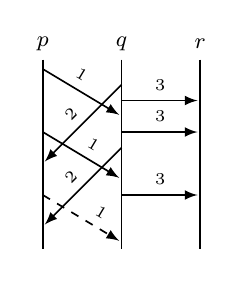
\begin{tikzpicture}[>=stealth,node distance=3.4cm,shorten >=1pt,
  every state/.style={text=black, scale =0.7}, semithick,
    font={\fontsize{8pt}{12}\selectfont}]
\begin{scope}[shift = {(0,0)}, scale = 0.8]
  % \draw (1.25, -4.75) node{\textbf{(a)}};
  % \draw (4.5, -4.75) node{\textbf(b)};

  %MACHINES
  \draw (0,-0.1) node{$p$} ;
  \draw (1.25,-0.1) node{$q$} ;
  \draw (2.5,-0.1) node{$r$} ;
  \draw (2.5, -0.35) -- (2.5, -3.4) ;
  \draw (0,-0.35) -- (0,-3.4) ;
  \draw (1.25,-0.35) -- (1.25,-3.4);
  %MESSAGES

  \draw[>=latex,->] (0, -0.5) -- (1.25, -1.25) node[pos=0.4, sloped, above] {$\amessage_1$};
  \draw[>=latex,->] (0, -1.5) -- (1.25, -2.25) node[pos=0.55, sloped, above] {$\amessage_1$};
  \draw[>=latex,->, dashed] (0, -2.5) -- (1.25, -3.25) node[pos=0.65, sloped, above] {$\amessage_1$};

  \draw[>=latex,->] (1.25, -0.75) -- (0, -2) node[pos=0.5, sloped, above] {$\amessage_2$};
  \draw[>=latex,->] (1.25, -1.75) -- (0, -3) node[pos=0.5, sloped, above] {$\amessage_2$};


  \draw[>=latex,->] (1.25, -1) -- (2.5, -1) node[midway, above] {$\amessage_3$};
  \draw[>=latex,->] (1.25, -1.5) -- (2.5, -1.5) node[midway, above] {$\amessage_3$};
  \draw[>=latex,->] (1.25, -2.5) -- (2.5, -2.5) node[midway, above] {$\amessage_3$};

  %\draw (0.6, -3.35) node{$\cdots$};
  %\draw (1.9, -3.35) node{$\cdots$};
\end{scope}
      % \begin{scope}[shift = {(3,0)}, scale = 0.8]
      %   % \draw (0.5, -4) node{\textbf{(b)}};
      %   %MACHINES
      %   \draw (0,0) node{$p$} ;
      %   \draw (1,0) node{$q$} ;
      %   \draw (0,-0.25) -- (0,-3.5) ;
      %   \draw (1,-0.25) -- (1,-3.5);
      %   %MESSAGES
      %
      %    \draw[>=latex,->] (0, -0.75) -- (1, -0.75) node[midway, above] {$\amessage_1$};
      %    \draw[>=latex,->] (1, -1.5) -- (0, -1.5) node[midway, above] {$\amessage_2$};
      %    \draw[>=latex,->] (0, -2.25) -- (1, -2.25) node[midway, above] {$\amessage_1$};
      %    \draw[>=latex,->] (1, -3) -- (0, -3) node[midway, above] {$\amessage_2$};
      %
      %
      %   % \draw (0.5, -3.25) node{$\cdots$};
      % \end{scope}
        \end{tikzpicture}
\captionof{figure}{MSC $\mscexist$}
\label{fig:msc_exist}
      \end{center}

% \end{minipage}
 \end{center}


By definition, \wks{k} systems are \wS{}.
Also, \sks{k} systems are included into \ekb{k} systems, as proved by Proposition~\ref{proposition:synchro_in_exists}, so \wks{k} are included into \ekb{k}.

We can see that \wS{} systems and \eb{} systems are incomparable. System
$\systemWSexist$ in Fig.~\ref{fig:system_W_S_exist} is \wS{}
%(and so \sS{})
because we
can send all messages before read them, and \ekb{1} because each MSC of
$\ppL{\systemWSexist}$ has a linearization of the form $\send{q}{p}{\msg_2} \cdot
(\send{p}{q}{\msg_1} \cdot \rec{p}{q}{\msg_1})^* \rec{q}{p}{\msg_2}$,  allowing
to have in each channel only one pending message.

\begin{center}
  \begin{minipage}[c]{6cm}
    \begin{center}
\begin{tikzpicture}[>=stealth,node distance=3.4cm,shorten >=1pt,
    every state/.style={text=black, scale =0.7}, semithick,
      font={\fontsize{8pt}{12}\selectfont}]
      \begin{scope}[->, shift={(0,0)}]
          \node[state,initial,initial text={}] (q0)  {$\ell_p^0$};
          \node[state, right of=q0] (q1)  {$\ell_p^1$};

          \path (q0) edge [loop above] node [right]   {$~\send{p}{q}{\msg_1}$}(q0);
          \path (q0) edge node [below] {$\rec{q}{r}{\msg_2}$} (q1);

          \node[rectangle, thick, draw] at (-0.7,0.6) {$A_p$};
      \end{scope}
      \begin{scope}[->, shift={(0,-1.5)}]
  	      \node[state,initial,initial text={}] (q0)  {$\ell_q^0$};
  				\node[state, right of=q0] (q1)  {$\ell_q^1$};

  				\path (q0) edge node [above] {$\send{q}{r}{\msg_2}$} (q1);
          \path (q1) edge [loop right] node [right]   {$\rec{p}{q}{\msg_1}~$}(q1);


      		\node[rectangle, thick, draw] at (-0.7,0.6) {$A_q$};
  	  \end{scope}
      \end{tikzpicture}
\captionof{figure}{System $\systemWSexist$}
\label{fig:system_W_S_exist}
      \end{center}

\end{minipage}
\hspace*{1cm}
\begin{minipage}[c]{3.5cm}
  \input{Appendix-Sec5/msc_W_S_exist}
\end{minipage}
\end{center}


But, system $\systemWS$ in
Fig.\ref{fig:system_W_S} is only \wS{}. Indeed, for each execution we can add an
iteration of message $\msg_1$ or $\msg_2$, or both, and, as we can see in
Fig.~\ref{fig:msc_W_S}, we need to send all
messages before begin to read, and so each execution need a bigger channel than
the previous one.
\begin{center}
  \begin{minipage}[c]{6cm}
\begin{center}
\begin{tikzpicture}[>=stealth,node distance=3.4cm,shorten >=1pt,
    every state/.style={text=black, scale =0.7}, semithick,
      font={\fontsize{8pt}{12}\selectfont}]
      \begin{scope}[->, shift={(0,0)}]
          \node[state,initial,initial text={}] (q0)  {$\ell_p^0$};
          \node[state, right of=q0] (q1)  {$\ell_p^1$};

          \path (q0) edge [loop above] node [right]   {$\send{p}{q}{\msg_1}$}(q0);
          \path (q0) edge node [below] {$\send{p}{q}{\msg_1}$} (q1);
          \path (q1)  edge [loop above] node [right] {$\rec{q}{p}{\msg_2}$} (q1);

          \node[rectangle, thick, draw] at (-0.7,0.6) {$A_p$};
      \end{scope}
      \begin{scope}[->, shift={(0,-2)}]
  	      \node[state,initial,initial text={}] (q0)  {$\ell_q^0$};
  				\node[state, right of=q0] (q1)  {$\ell_q^1$};

          \path (q0) edge [loop above] node [right]   {$\send{q}{p}{\msg_2}$}(q0);
          \path (q0) edge node [below] {$\send{q}{p}{\msg_2}$} (q1);
          \path (q1)  edge [loop above] node [right] {$\rec{p}{q}{\msg_1}$} (q1);


      		\node[rectangle, thick, draw] at (-0.7,0.6) {$A_q$};
  	  \end{scope}
      \end{tikzpicture}
\captionof{figure}{System $\systemWS$}
\label{fig:system_W_S}
      \end{center}

\end{minipage}
\hspace*{1cm}
\begin{minipage}[c]{3.5cm}
\begin{center}
  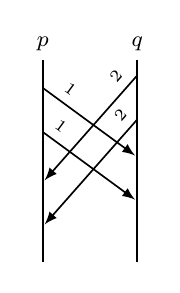
\begin{tikzpicture}[>=stealth,node distance=3.4cm,shorten >=1pt,
  every state/.style={text=black, scale =0.7}, semithick,
    font={\fontsize{8pt}{12}\selectfont}]

\begin{scope}[shift = {(8,0.75)}, scale = 0.8]
%	\draw (0.75, -4) node{\textbf{(b)}};
  %MACHINES
  \draw (0,0) node{$p$} ;
  \draw (1.5,0) node{$q$} ;
  \draw (0,-0.25) -- (0,-3.5) ;
  \draw (1.5,-0.25) -- (1.5,-3.5);
  %MESSAGES

  \draw[>=latex,->] (0, -0.7) -- (1.5, -1.8) node[pos=0.2, sloped, above] {$\amessage_1$};
  \draw[>=latex,->] (0, -1.4) -- (1.5, -2.5) node[pos=0.1, sloped, above] {$\amessage_1$}; %{$\amessage_1'$};
  %\draw[>=latex,->, dashed] (0, -2.5) -- (1.25, -3.25) node[pos=0.55, sloped, above] {$\amessage_1''$};

  \draw[>=latex,->] (1.5, -0.5) -- (0, -2.2) node[pos=0.1, sloped, above] {$\amessage_2$};
  \draw[>=latex,->] (1.5, -1.2) -- (0, -2.9) node[pos=0.05, sloped, above] {$\amessage_2$};
  % \node[rotate = 90, left]at (1.13, -0.65) {$\cdots$};
  % \node[rotate = -90, right]at (0.1, -0.65) {$\cdots$};

\end{scope}

\end{tikzpicture}
\captionof{figure}{MSC $\mscWS$}
\label{fig:msc_W_S}
\end{center}

\end{minipage}
\end{center}

For system $\systemuniver$ in Fig.~\ref{fig:system_univer}, we
can see an example of MSC in Fig.~\ref{fig:msc_univer} which cannot be divided
into exchanges as send and receptions are intertwined and so $\systemuniver$ is not
\wS{}.

\begin{center}
  \begin{minipage}[c]{6cm}
    
  \begin{center}
      \begin{tikzpicture}[>=stealth,node distance=3.4cm,shorten >=1pt,
      every state/.style={text=black, scale =0.65}, semithick,
        font={\fontsize{8pt}{12}\selectfont}]
    \begin{scope}[->]
	      \node[state,initial,initial text={}] (q0)  {$\ell_p^0$};
	      \node[state, right of=q0] (q1)  {$\ell_p^1$};
				\node[state, right of=q1] (q2) {$\ell_p^2$};

	    	\path (q0) edge node [above] {$\send{p}{q}{\msg_1}$} (q1);
				\path (q1) edge[bend left = 10] node [above] {$\send{p}{q}{\msg_1}$}(q2);
				\path (q2) edge[bend left = 10] node [below] {$\rec{q}{p}{\msg_2}$}(q1);

	    	\node[rectangle, thick, draw] at (-0.7,0.5) {$A_p$};
	  \end{scope}

		\begin{scope}[->, shift={(0,-1.5)}]
	      \node[state,initial,initial text={}] (q0)  {$\ell_q^0$};
				\node[state, right of=q0] (q1)  {$\ell_q^1$};

				\path (q0) edge[bend left = 10] node [above] {$\send{q}{p}{\msg_2}$} (q1);
        \path (q1) edge[bend left = 10] node [below] {$\rec{p}{q}{\msg_1}$} (q0);

    		\node[rectangle, thick, draw] at (-0.7,0.5) {$A_q$};


	  \end{scope}

	\end{tikzpicture}
	\captionof{figure}{System $\systemuniver$ }
	\label{fig:system_univer}

  \end{center}

\end{minipage}
\hspace*{1cm}
\begin{minipage}[c]{3.5cm}
  \begin{center}
  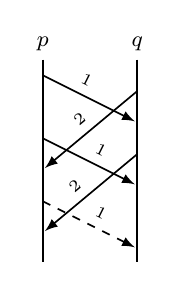
\begin{tikzpicture}[>=stealth,node distance=3.4cm,shorten >=1pt,
  every state/.style={text=black, scale =0.7}, semithick,
    font={\fontsize{8pt}{12}\selectfont}]

\begin{scope}[shift = {(8,0.75)}, scale = 0.8]
%	\draw (0.75, -4) node{\textbf{(b)}};
  %MACHINES
  \draw (0,0) node{$p$} ;
  \draw (1.5,0) node{$q$} ;
  \draw (0,-0.25) -- (0,-3.5) ;
  \draw (1.5,-0.25) -- (1.5,-3.5);
  %MESSAGES

  \draw[>=latex,->] (0, -0.5) -- (1.5, -1.25) node[pos=0.4, sloped, above] {$\amessage_1$};
  \draw[>=latex,->] (0, -1.5) -- (1.5, -2.25) node[pos=0.55, sloped, above] {$\amessage_1$};
  \draw[>=latex,->, dashed] (0, -2.5) -- (1.5, -3.25) node[pos=0.55, sloped, above] {$\amessage_1$};


  \draw[>=latex,->] (1.5, -0.75) -- (0, -2) node[pos=0.5, sloped, above] {$\amessage_2$};
  \draw[>=latex,->] (1.5, -1.75) -- (0, -3) node[pos=0.55, sloped, above] {$\amessage_2$};
%  \draw (0.6, -3.25) node{$\cdots$};

\end{scope}

\end{tikzpicture}
\captionof{figure}{MSC $\mscuniver$}
\label{fig:msc_univer}
\end{center}

\end{minipage}
\end{center}




We can observe that $\systemuniver$ is \ukb{3} as each time a
message is sent, one is received and
the maximal number of messages in a buffer is 3. As we said, $\systemWS$ is \wS{} but not \eb{} and so not \ub{}, so \wS{} and \ub{} systems are incomparable.
However, as proved in Proposition~\ref{proposition:weak_univer_uweak}, a system which is both is also \wks{k} (not necessarly for the same $k$).

Finally, \wks{k} and \ukb{k} systems are incomparable. System $\systemweakuniver$ in
Fig.~\ref{fig:system_weak_univer} is  both weakly 1-synchronizable and
universally 1-bounded.   But,  we have, for example, system $\systemweakSexist$ below
which is \wks{1} but not \ukb{k} for any $k$.  Indeed,
each execution can be rescheduled to have all the receptions just after the
respective sends. Then each MSC can be divided into \kE{1}s  (for an example,
see  MSC $\mscweakSexist$ in Fig.~\ref{fig:msc_weak_S_exist}). However, as we can send an
unbounded number of $\msg_2$ messages before reading them, the size of channel
$c_p$ can also be unbounded thus the system is not universally bounded.
Conversely, as we have seen, system $\systemuniver$ is \ukb{3} but not \wks{k} for any $k$.

%\begin{figure}
  \begin{center}

  \begin{tikzpicture}[>=stealth,node distance=3.5cm,shorten >=1pt,
      every state/.style={text=black, scale =0.65}, semithick,
      font={\fontsize{8pt}{12}\selectfont}]
	% %P
	  \begin{scope}[->]
	      \node[state,initial,initial text={}] (q0)  {$\ell_p^0$};
	      \node[state, right of=q0] (q1)  {$\ell_p^1$};
				\node[state, right of=q1] (q2) {$\ell_p^2$};

	    	\path (q0) edge node [below] {$\send{p}{q}{\msg_1}$} (q1);
				\path (q1) edge node [below] {$\rec{q}{p}{\msg_2}$}(q2);
				\path (q2) edge [loop above] node [above]   {$~\rec{q}{p}{\msg_2}$}(q2);

	    	\node[rectangle, thick, draw] at (-0.7,0.4) {$A_p$};
	  \end{scope}

	  \begin{scope}[->, shift={(6.5,0)} ]
	      \node[state,initial,initial text={}] (q0)  {$\ell_q^0$};
				\node[state, right of=q0] (q1)  {$\ell_q^1$};
				\node[state, right of=q1] (q2) {$\ell_q^2$};

				\path (q0) edge node [below] {$\send{q}{p}{\msg_2}$} (q1);
				\path (q1) edge [loop above] node [above]   {$~\send{q}{p}{\msg_2}$}(q1);
				\path (q1) edge node [below] {$\rec{r}{q}{\msg_3}$}(q2);
				\node[rectangle, thick, draw] at (-0.7,0.4) {$A_q$};
	  \end{scope}

		\begin{scope}[->, shift={(4.5,-1.3)} ]
	      \node[state,initial,initial text={}] (q0)  {$\ell_r^0$};
				\node[state, right of=q0] (q1)  {$\ell_r^1$};

				\path (q0) edge node [below] {$\send{r}{q}{\msg_3}$} (q1);
				\node[rectangle, thick, draw] at (-0.7,0.4) {$A_r$};
			%\node at (1, -.7) {\textbf{(a)}};

	  \end{scope}
		% \begin{scope}[shift = {(8,0.5)}, scale = 0.8]
		% 	\draw (1, -4.25) node{\textbf{(b) existe plus haut}};
    %   \node at (-9, -4.25) {\textbf{(a)}};
    %
		% 	%MACHINES
		% 	\draw (0,0) node{$p$} ;
		% 	\draw (1,0) node{$q$} ;
		% 	\draw (2,0) node{$r$} ;
		% 	\draw (0,-0.25) -- (0,-3.5) ;
		% 	\draw (1,-0.25) -- (1,-3.5);
		% 	\draw (2, -0.25) -- (2, -3.5) ;
		% 	%MESSAGES
		% 	\draw[>=latex,->, dashed] (0,-0.75) -- (1, -0.75) node[midway,above]{$\amessage_1$};
    %
		% 	\draw[>=latex,->] (1, -1.5) -- (0, -1.5) node[midway, above] {$\amessage_2$};
		% 	\draw (0.5,-1.7) node{$\cdots$};
		% 	\draw[>=latex,->] (1, -2.25) -- (0, -2.25) node[midway, above] {$\amessage_2$};
    %
		% 	\draw[>=latex,->] (2,-3) -- (1,-3) node[midway, above] {$\amessage_3$};
		% \end{scope}
\end{tikzpicture}
\captionof{figure}{System $\systemweakSexist$}
\label{fig:system_weak_S_exist}

\end{center}
%\end{figure}



\subsubsection{Mailbox systems }

Now consider  mailbox semantics. As depicted in Fig. \ref{fig:diagram_mailbox_all}, we can now distinguish between weakly and strongly synchronizable systems.

Some inclusions are obvious, by definition of the classes:
\begin{itemize}
  \item \ub{} systems are \eb{}, but it is a proper inclusion. Indeed, a system, as system $\systemexist$ in Fig.~\ref{fig:system_exist}, can be \ekb{1}, but not \ub{}. In this case, as in \pp semantics, an unbounded number of message $\msg_3$ can be sent before be read, as we can see in MSC $\mscexist$ in Fig.~\ref{fig:msc_exist}.
  \item \sks{k} systems are \sS{}. As well, a system can be \sS{} without have a bound on the size of its exchange, as system $\systemWS$ in Fig~\ref{fig:system_W_S}. See an example of MSC of $\systemWS$ in Fig~\ref{fig:msc_W_S}, where we can always build a bigger exchange adding iterations of messages $\msg_1$ or $\msg_2$.
  \item \wks{k} systems are \wS{}. We can also find a \wS{} system without bound on the size of its exchange. Let see $\systemW$ in Fig.~\ref{fig:system_W} with MSC $\mscW$ in Fig.~\ref{fig:msc_W}, which can be divided into exchanges, each message can be in a separate exchange, except messages $\msg_2$ and $\msg_3$ that have to be all in the same exchange. As we can have as many repetitions of them, this exchange no have bound on its size and prevent the system to be \wks{k} for a precise $k$.
\end{itemize}




%
% \begin{center}
%   \begin{minipage}[c]{6cm}
     
\begin{center}
\begin{tikzpicture}[>=stealth,node distance=3.4cm,shorten >=1pt,
    every state/.style={text=black, scale =0.7}, semithick,
      font={\fontsize{8pt}{12}\selectfont}]
      \begin{scope}[->, shift={(0,0)}]
          \node[state,initial,initial text={}] (q0)  {$\ell_p^0$};
          \node[state, right of=q0] (q1)  {$\ell_p^1$};
          \node[state, right of=q1] (q2)  {$\ell_p^2$};


          \path (q0) edge node [above] {$\send{p}{q}{\msg_1}$} (q1);
          \path (q1) edge node [above]  {$\rec{q}{p}{\msg_2}$} (q2);

          \node[rectangle, thick, draw] at (-0.7,0.6) {$A_p$};
      \end{scope}
      \begin{scope}[->, shift={(7,0)}]
  	      \node[state,initial,initial text={}] (q0)  {$\ell_q^0$};
  				\node[state, right of=q0] (q1)  {$\ell_q^1$};
          \node[state, right of=q1] (q2)  {$\ell_q^2$};

          \path (q0) edge [loop above] node [right]   {$\send{q}{r}{\msg_3}$}(q0);
          \path (q0) edge node [above] {$\send{q}{r}{\msg_3}$} (q1);
          \path (q1) edge [loop above] node [right]   {$\rec{r}{q}{\msg_4}$}(q1);
          \path (q1) edge node [above] {$\rec{r}{q}{\msg_5}$} (q2);

      		\node[rectangle, thick, draw] at (-0.7,0.6) {$A_q$};
  	  \end{scope}

      \begin{scope}[->, shift={(3.5,-1.5)}]
          \node[state,initial,initial text={}] (q0)  {$\ell_q^0$};
          \node[state, right of=q0] (q1)  {$\ell_q^1$};
          \node[state, right of=q1] (q2)  {$\ell_q^2$};


          \path (q0) edge node [above] {$\send{r}{q}{\msg_4}$} (q1);
          \path (q0) edge [loop above] node [right]  {$\send{r}{q}{\msg_4}$}(q0);

          \path (q1) edge [loop above] node [right]  {$\rec{q}{r}{\msg_3}$}(q1);
          \path (q1) edge node [above] {$\send{r}{q}{\msg_5}$} (q2);

          \node[rectangle, thick, draw] at (-0.7,0.6) {$A_r$};
      \end{scope}
      \end{tikzpicture}
\captionof{figure}{System $\systemW$}
\label{fig:system_W}
      \end{center}

% \end{minipage}
% \hspace*{1cm}
% \begin{minipage}[c]{3.5cm}
%   \begin{center}
  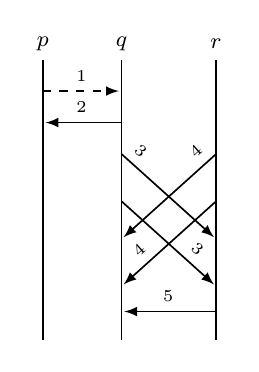
\begin{tikzpicture}[>=stealth,node distance=3.4cm,shorten >=1pt,
  every state/.style={text=black, scale =0.7}, semithick,
    font={\fontsize{8pt}{12}\selectfont}]

\begin{scope}[shift = {(8,0.75)}, scale = 0.8]
%	\draw (0.75, -4) node{\textbf{(b)}};
  %MACHINES
  \draw (0,1.25) node{$q$} ;
  \draw (1.5,1.25) node{$r$} ;
  \draw (-1.25,1.25) node{$p$} ;
  \draw (0,1) -- (0,-3.5) ;
  \draw (1.5,1) -- (1.5,-3.5);
  \draw (-1.25,1) -- (-1.25,-3.5);

  %MESSAGES
  \draw[>=latex,->, dashed] (-1.25, 0.5) -- (0, 0.5) node[ above, midway] {$\amessage_1$};
  \draw[>=latex,->] (0, 0) -- (-1.25, 0) node[ above, midway] {$\amessage_2$};


  \draw[>=latex,->] (0, -0.5) -- (1.5, -1.85) node[pos=0.1, sloped, above] {$\amessage_3$};
  \draw[>=latex,->] (0, -1.25) -- (1.5, -2.6) node[pos=0.7, sloped, above] {$\amessage_3$}; %{$\amessage_1'$};
  %\draw[>=latex,->, dashed] (0, -2.5) -- (1.25, -3.25) node[pos=0.55, sloped, above] {$\amessage_1''$};

  \draw[>=latex,->] (1.5, -0.5) -- (0, -1.85) node[pos=0.1, sloped, above] {$\amessage_4$};
  \draw[>=latex,->] (1.5, -1.25) -- (0, -2.6) node[pos=0.7, sloped, above] {$\amessage_4$}; %{$\amessage_2'$};
  %\node[rotate = 90, left]at (1.13, -0.65) {$\cdots$};
  %\node[rotate = -90, right]at (0.1, -0.65) {$\cdots$};

  \draw[>=latex,->] (1.5, -3) -- (0, -3) node[ above, midway] {$\amessage_5$};


\end{scope}

\end{tikzpicture}
\captionof{figure}{MSC $\msc_{2}$}
\label{fig:msc_W}
\end{center}

% \end{minipage}
% \end{center}


The classes of \wS{} and \wks{k} systems are incomparable with the classes of \eb{} and \ub{} systems.

Indeed, let see system $\systemuniver$ in Fig.~\ref{fig:system_univer} which is \ukb{3}. It cannot be \wS{} (and so \wks{k} for a $k$) as we cannot divide a corresponding MSC, as $\mscuniver$ in Fig.~\ref{fig:msc_univer}, into exchanges, where all sends have to be before all receptions, as in \pp semantics.
We see a difference with the \pp semantics looking at $\systemweak$ in
Fig.~\ref{fig:system_weak} which is \wS{} but not \eb{}. Indeed, we can see in
Fig.~\ref{fig:msc_weak} that $\mscweak$ can be divided easily into \kE{1} but,
as $\msg_1$ has to be sent before $\msg_4$, and $\msg_2$ has to be sent to send
$\msg_4$,  it means  that all messages $\msg_2$ have to wait the send of
$\msg_4$ to be read.  Then, each execution is $x$-mailbox-bounded, where $x$ is
the number of repetitions of $\msg_2$. Then, there is no bound on the buffers
and $\systemweak$ cannot be \eb{} (and so \ub{}).



\begin{center}
  \begin{minipage}[c]{6cm}
    
  \begin{center}

  \begin{tikzpicture}[>=stealth,node distance=3.4cm,shorten >=1pt,
      every state/.style={text=black, scale =0.65}, semithick,
        font={\fontsize{8pt}{12}\selectfont}]

        \begin{scope}[-> ]
            \node[state,initial,initial text={}] (q0)  {$\ell_p^0$};
            \node[state, right of=q0] (q1)  {$\ell_p^1$};
            \node[state, right of=q1] (q2) {$\ell_p^2$};

            \path (q0) edge node [above] {$\send{p}{q}{\msg_2}$} (q1);
            \path (q1) edge [loop above] node [right]   {$~\send{p}{q}{\msg_2}$}(q1);
            \path (q1) edge node [above] {$\send{p}{s}{\msg_3}$}(q2);
            \node[rectangle, thick, draw] at (-0.6,0.6) {$A_p$};
        \end{scope}


      \begin{scope}[->,  shift={(0,-1.1)}]
          \node[state,initial,initial text={}] (q0)  {$\ell_q^0$};
          \node[state, right of=q0] (q1)  {$\ell_q^1$};
          \node[state, right of=q1] (q2) {$\ell_q^2$};

          \path (q0) edge node [above] {$\send{q}{r}{\msg_1}$} (q1);
          \path (q1) edge node [above] {$\rec{p}{q}{\msg_2}$}(q2);
          \path (q2) edge [loop above] node [right]   {$~\rec{p}{q}{\msg_2}$}(q2);

          \node[rectangle, thick, draw] at (-0.6,0.6) {$A_q$};
      \end{scope}



      \begin{scope}[->, shift={(0,-2.2)} ]
          \node[state,initial,initial text={}] (q0)  {$\ell_r^0$};
          \node[state, right of=q0] (q1)  {$\ell_r^1$};

          \path (q0) edge node [above] {$\rec{s}{r}{\msg_4}$} (q1);

          \node[rectangle, thick, draw] at (-0.6,0.6) {$A_r$};
        %\node at (1, -1.5) {\textbf{(a)}};

      \end{scope}
      \begin{scope}[->, shift ={(0, -3.3)}]
         \node[state,initial,initial text={}] (q0)  {$\ell_s^0$};
         \node[state, right of=q0] (q1)  {$\ell_s^1$};
         \node[state, right of=q1] (q2) {$\ell_s^2$};

         \path (q0) edge node [above] {$\rec{p}{s}{\msg_3}$} (q1);
         \path (q1) edge node [above] {$\send{s}{r}{\msg_4}$} (q2);

         \node[rectangle, thick, draw] at (-0.6,0.6) {$A_s$};

      \end{scope}
      % \begin{scope}[shift = {(8.5,0)}, scale = 0.8]
      %   \draw (1.5, -4.75) node{\textbf{(b)}};
      %   \draw (-9.5, -4.75) node{\textbf{(a)}};
      %
      %   %MACHINES
      %   \draw (0,0) node{$p$} ;
    	% 	\draw (1,0) node{$q$} ;
    	% 	\draw (2,0) node{$r$} ;
      %   \draw (3,0) node{$s$} ;
    	% 	\draw (0,-0.25) -- (0,-3.75) ;
    	% 	\draw (1,-0.25) -- (1,-3.75);
    	% 	\draw (2, -0.25) -- (2, -3.75) ;
      %   \draw (3, -0.25) -- (3, -3.75) ;
      %
    	% 	%MESSAGES
    	% 	\draw[>=latex,->, dashed] (1,-0.7) -- (2, -0.7) node[midway,above]{$\amessage_1$};
      %
    	% 	\draw[>=latex,->] (0, -1.35) -- (1, -1.35) node[midway, above] {$\amessage_2$};
      %
    	% 	\draw[>=latex,->] (0,-2.1) -- (1,-2.1) node[midway, above] {$\amessage_2$};
      %
    	% 	\draw[>=latex,->] (0,-2.75) -- (3,-2.75) node[midway,above] {$\amessage_3$};
      %
      %   \draw[>=latex,->] (3,-3.4) -- (2,-3.4) node[midway,above] {$\amessage_4$};
      %
      % %  \draw[>=latex,->] (2,-3.25) -- (3,-3.25) node[midway,above] {$\amessage_5$};
      %
      %   \draw (0.5, -1.55) node{$\cdots$};
      %
      % \end{scope}


  \end{tikzpicture}
  \captionof{figure}{System $\systemweak$ }
  \label{fig:system_weak}

\end{center}

\end{minipage}
\hspace*{1cm}
\begin{minipage}[c]{3.5cm}
  \begin{center}


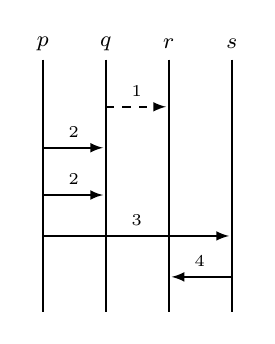
\begin{tikzpicture}[>=stealth,node distance=3.4cm,shorten >=1pt,
    every state/.style={text=black, scale =0.7}, semithick,
      font={\fontsize{8pt}{12}\selectfont}]

\begin{scope}[shift = {(8.5,0)}, scale = 0.8]

  %MACHINES
  \draw (0,0.3) node{$p$} ;
  \draw (1,0.3) node{$q$} ;
  \draw (2,0.3) node{$r$} ;
  \draw (3,0.3) node{$s$} ;
  \draw (0,0.05) -- (0,-4) ;
  \draw (1,0.05) -- (1,-4);
  \draw (2, 0.05) -- (2, -4) ;
  \draw (3, 0.05) -- (3, -4) ;

  %MESSAGES
  \draw[>=latex,->, dashed] (1,-0.7) -- (2, -0.7) node[midway,above]{$\amessage_1$};

  \draw[>=latex,->] (0, -1.35) -- (1, -1.35) node[midway, above] {$\amessage_2$};

  \draw[>=latex,->] (0,-2.1) -- (1,-2.1) node[midway, above] {$\amessage_2$};

  \draw[>=latex,->] (0,-2.75) -- (3,-2.75) node[midway,above] {$\amessage_3$};

  \draw[>=latex,->] (3,-3.4) -- (2,-3.4) node[midway,above] {$\amessage_4$};

%  \draw[>=latex,->] (2,-3.25) -- (3,-3.25) node[midway,above] {$\amessage_5$};

  %\draw (0.5, -1.55) node{$\cdots$};

\end{scope}
\end{tikzpicture}
\captionof{figure}{MSC $\mscweak$ }
\label{fig:msc_weak}
\end{center}

\end{minipage}
\end{center}


Finally, as proved in Proposition~\ref{proposition:weak_univer_uweak}, if a system is \wS{} and \ub{} system, there is a $k$ such that it is also \sks{k}. In all the other intersections, we can find a system:
\begin{itemize}
  \item \wS{} and \eb{} (but not \wks{k} or \ub{}): $\systemWexist$ in Fig.~\ref{fig:system_W_exist} is \ekb{1} but there is no bound on the size of the exchange containing messages $\msg_3$ and $\msg_4$ and so $\systemWexist$ cannot be \wks{k}, and repetitions of $\msg_3$ prevent it to be \ub{};
\end{itemize}
  \begin{center}
    \begin{minipage}[c]{6cm}
      
\begin{center}
\begin{tikzpicture}[>=stealth,node distance=3.4cm,shorten >=1pt,
    every state/.style={text=black, scale =0.7}, semithick,
      font={\fontsize{8pt}{12}\selectfont}]
      \begin{scope}[->, shift={(7,0)}]
          \node[state,initial,initial text={}] (q0)  {$\ell_p^0$};
          \node[state, right of=q0] (q1)  {$\ell_p^1$};
          \node[state, right of=q1] (q2)  {$\ell_p^2$};


          \path (q0) edge node [above] {$\send{p}{q}{\msg_1}$} (q1);
          \path (q1) edge node [above]  {$\rec{q}{p}{\msg_2}$} (q2);

          \node[rectangle, thick, draw] at (-0.7,0.6) {$A_p$};
      \end{scope}
      \begin{scope}[->, shift={(7,-1.5)}]
  	      \node[state,initial,initial text={}] (q0)  {$\ell_q^0$};
  				\node[state, right of=q0] (q1)  {$\ell_q^1$};
          \node[state, right of=q1] (q2)  {$\ell_q^2$};

          \path (q0) edge [loop above] node [right]   {$\send{q}{r}{\msg_3}$}(q0);
          \path (q0) edge node [above] {$\rec{r}{q}{\msg_4}$} (q1);
          \path (q1) edge node [above] {$\rec{r}{q}{\msg_5}$} (q2);

      		\node[rectangle, thick, draw] at (-0.7,0.6) {$A_q$};
  	  \end{scope}

      \begin{scope}[->, shift={(7,-3)}]
          \node[state,initial,initial text={}] (q0)  {$\ell_q^0$};
          \node[state, right of=q0] (q1)  {$\ell_q^1$};
          \node[state, right of=q1] (q2)  {$\ell_q^2$};


          \path (q0) edge node [above] {$\send{r}{q}{\msg_4}$} (q1);
          \path (q1) edge [loop above] node [right]  {$\rec{q}{r}{\msg_3}$}(q1);
          \path (q1) edge node [above] {$\send{r}{q}{\msg_5}$} (q2);

          \node[rectangle, thick, draw] at (-0.7,0.6) {$A_q$};
      \end{scope}
      \end{tikzpicture}
\captionof{figure}{System $\systemWexist$}
\label{fig:system_W_exist}
      \end{center}

  \end{minipage}
  \hspace*{1cm}
  \begin{minipage}[c]{3.5cm}
    \begin{center}
  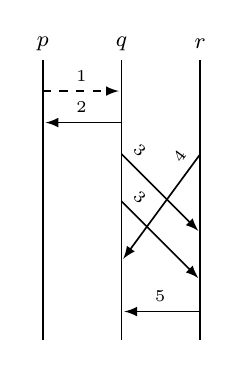
\begin{tikzpicture}[>=stealth,node distance=3.4cm,shorten >=1pt,
  every state/.style={text=black, scale =0.7}, semithick,
    font={\fontsize{8pt}{12}\selectfont}]

\begin{scope}[shift = {(8,0.75)}, scale = 0.8]
%	\draw (0.75, -4) node{\textbf{(b)}};
  %MACHINES
  \draw (0,1.25) node{$q$} ;
  \draw (1.25,1.25) node{$r$} ;
  \draw (-1.25,1.25) node{$p$} ;
  \draw (0,1) -- (0,-3.5) ;
  \draw (1.25,1) -- (1.25,-3.5);
  \draw (-1.25,1) -- (-1.25,-3.5);

  %MESSAGES
  \draw[>=latex,->, dashed] (-1.25, 0.5) -- (0, 0.5) node[ above, midway] {$\amessage_1$};
  \draw[>=latex,->] (0, 0) -- (-1.25, 0) node[ above, midway] {$\amessage_2$};


  \draw[>=latex,->] (0, -0.5) -- (1.25, -1.75) node[pos=0.1, sloped, above] {$\amessage_3$};
  \draw[>=latex,->] (0, -1.25) -- (1.25, -2.5) node[pos=0.1, sloped, above] {$\amessage_3$}; %{$\amessage_1'$};
  %\draw[>=latex,->, dashed] (0, -2.5) -- (1.25, -3.25) node[pos=0.55, sloped, above] {$\amessage_1''$};

  \draw[>=latex,->] (1.25, -0.5) -- (0, -2.2) node[pos=0.1, sloped, above] {$\amessage_4$};
%  \draw[>=latex,->] (1.25, -1.25) -- (0, -2.5) node[pos=0.55, sloped, above] {}; %{$\amessage_2'$};
%  \node[rotate = 90, left]at (1.13, -0.65) {$\cdots$};
  %\node[rotate = -90, right]at (0.1, -0.65) {$\cdots$};

  \draw[>=latex,->] (1.25, -3) -- (0, -3) node[ above, midway] {$\amessage_5$};


\end{scope}

\end{tikzpicture}
\captionof{figure}{MSC $\mscWexist$}
\label{fig:msc_W_exist}
\end{center}

  \end{minipage}
  \end{center}
  \begin{itemize}
      \item \wks{k} and \eb{} (but not \ub{}): $\systemweakexist$ in Fig.~\ref{fig:system_weak_exist} is \wks{1} and \ekb{1} but repetitions of $\msg_3$ prevent it from being \ub{};
  \end{itemize}
  \begin{center}
    \begin{minipage}[c]{6cm}
      

\begin{center}
\begin{tikzpicture}[>=stealth,node distance=3.4cm,shorten >=1pt,
    every state/.style={text=black, scale =0.7}, semithick,
      font={\fontsize{8pt}{12}\selectfont}]
      \begin{scope}[->, shift={(7,0)}]
          \node[state,initial,initial text={}] (q0)  {$\ell_p^0$};
          \node[state, right of=q0] (q1)  {$\ell_p^1$};
          \node[state, right of=q1] (q2)  {$\ell_p^2$};


          \path (q0) edge node [above] {$\send{p}{q}{\msg_1}$} (q1);
          \path (q1) edge node [above]  {$\rec{q}{p}{\msg_2}$} (q2);

          \node[rectangle, thick, draw] at (-0.7,0.6) {$A_p$};
      \end{scope}
      \begin{scope}[->, shift={(7,-1.5)}]
  	      \node[state,initial,initial text={}] (q0)  {$\ell_q^0$};
  				\node[state, right of=q0] (q1)  {$\ell_q^1$};
          \node[state, right of=q1] (q2)  {$\ell_q^2$};

          \path (q1) edge [loop above] node [right]   {$\send{q}{r}{\msg_3}$}(q1);
          \path (q0) edge node [above] {$\send{q}{p}{\msg_2}$} (q1);
          \path (q1) edge node [above] {$\rec{r}{q}{\msg_4}$} (q2);

      		\node[rectangle, thick, draw] at (-0.7,0.6) {$A_q$};
  	  \end{scope}

      \begin{scope}[->, shift={(7,-3)}]
          \node[state,initial,initial text={}] (q0)  {$\ell_q^0$};
          \node[state, right of=q0] (q1)  {$\ell_q^1$};


          \path (q0) edge [loop above] node [right]  {$\rec{q}{r}{\msg_3}$}(q0);
          \path (q0) edge node [above] {$\send{r}{q}{\msg_4}$} (q1);

          \node[rectangle, thick, draw] at (-0.7,0.6) {$A_q$};
      \end{scope}
      \end{tikzpicture}
\captionof{figure}{System $\systemweakexist$}
\label{fig:system_weak_exist}
      \end{center}

  \end{minipage}
  \hspace*{1cm}
  \begin{minipage}[c]{3.5cm}
    \begin{center}
  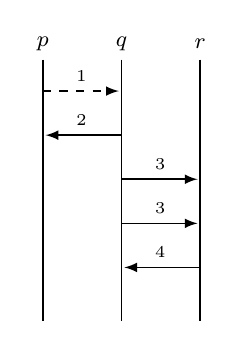
\begin{tikzpicture}[>=stealth,node distance=3.4cm,shorten >=1pt,
  every state/.style={text=black, scale =0.7}, semithick,
    font={\fontsize{8pt}{12}\selectfont}]

\begin{scope}[shift = {(8,0.75)}, scale = 0.8]
%	\draw (0.75, -4) node{\textbf{(b)}};
  %MACHINES
  \draw (0,1.25) node{$q$} ;
  \draw (1.25,1.25) node{$r$} ;
  \draw (-1.25,1.25) node{$p$} ;
  \draw (0,1) -- (0,-3.2) ;
  \draw (1.25,1) -- (1.25,-3.2);
  \draw (-1.25,1) -- (-1.25,-3.2);

  %MESSAGES
  \draw[>=latex,->, dashed] (-1.25, 0.5) -- (0, 0.5) node[ above, midway] {$\amessage_1$};
  \draw[>=latex,->] (0, -0.2) -- (-1.25, -0.2) node[ above, midway] {$\amessage_2$};


  \draw[>=latex,->] (0, -0.9) -- (1.25, -0.9) node[midway, sloped, above] {$\amessage_3$};
  \draw[>=latex,->] (0, -1.6) -- (1.25, -1.6) node[midway, sloped, above] {$\amessage_3$}; %{$\amessage_1'$};
  %\draw[>=latex,->, dashed] (0, -2.5) -- (1.25, -3.25) node[pos=0.55, sloped, above] {$\amessage_1''$};

  %\draw[>=latex,->] (1.25, -0.5) -- (0, -1.75) node[pos=0.1, sloped, above] {$\amessage_4$};
%  \draw[>=latex,->] (1.25, -1.25) -- (0, -2.5) node[pos=0.55, sloped, above] {}; %{$\amessage_2'$};
%  \node[rotate = 90, left]at (1.13, -0.65) {$\cdots$};
%  \node[rotate = -90, right]at (0.1, -0.65) {$\cdots$};

  \draw[>=latex,->] (1.25, -2.3) -- (0, -2.3) node[ above, midway] {$\amessage_4$};


\end{scope}

\end{tikzpicture}
\captionof{figure}{MSC $\mscweakexist$}
\label{fig:msc_weak_exist}
\end{center}

  \end{minipage}
  \end{center}
\begin{itemize}
  \item \wks{k} and \ub{} as $\systemuniver$ in Fig.~\ref{fig:system_weak_univer}.

\end{itemize}







Now, focus on the strong classes. We know by
Proposition~\ref{proposition:synchro_in_exists} that a \sks{k} is \eb{}. So let
compare \sks{k} systems with \ub{} ones.  We can see that there are incomparable.
$\systemstrongexist$ in Fig.~\ref{fig:system_strong_exist} is \sks{1}, as we can
see with $\mscstrongexist$ in Fig.~\ref{fig:msc_strong_exist}, but cannot be \ub{} as
the unbounded iterations of $\msg_1$ can be stored before begin to read.
As we see before $\System_7$ is only \ub{} and cannot have any synchronizable property. But, $\systemstronguniver$ in Fig.~\ref{fig:system_strong_univer} is both \sks{1} and \ukb{1}.

% \begin{center}
%   % \begin{minipage}[c]{6cm}
%
% % \end{minipage}
% % \hspace*{1cm}
% % \begin{minipage}[c]{3.5cm}
% %   \begin{center}

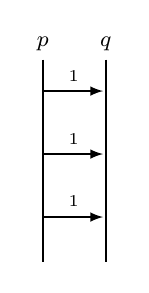
\begin{tikzpicture}[>=stealth,node distance=3.4cm,shorten >=1pt,
    every state/.style={text=black, scale =0.7}, semithick,
      font={\fontsize{8pt}{12}\selectfont}]

      \begin{scope}[shift = {(3.5,0.75)}, scale = 0.8]
           %\draw (0.5, -4) node{\textbf{(b)}};
          %MACHINES
          \draw (0,0) node{$p$} ;
          \draw (1,0) node{$q$} ;
          \draw (0,-0.25) -- (0,-3.5) ;
          \draw (1,-0.25) -- (1,-3.5);
          %MESSAGES

           \draw[>=latex,->] (0, -0.75) -- (1, -0.75) node[midway, above] {$\amessage_1$};
           \draw[>=latex,->] (0, -1.75) -- (1, -1.75) node[midway, above] {$\amessage_1$};
           \draw[>=latex,->] (0, -2.75) -- (1, -2.75) node[midway, above] {$\amessage_1$};

           %\draw (0.5, -3.25) node{$\cdots$};
      \end{scope}

\end{tikzpicture}
\captionof{figure}{MSC $\mscstrongexist$}
\label{fig:msc_strong_exist}
\end{center}

% % \end{minipage}
% \end{center}


% \begin{center}
%   \begin{center}

  \begin{tikzpicture}[>=stealth,node distance=3.4cm,shorten >=1pt,
      every state/.style={text=black, scale =0.65}, semithick,
        font={\fontsize{8pt}{12}\selectfont}]


      \begin{scope}[->, shift={(0,0)}]
          \node[state,initial,initial text={}] (q0)  {$\ell_p^0$};
           \path (q0) edge [loop right] node [right]   {$~\send{p}{q}{\msg_1}$}(q0);
          \node[rectangle, thick, draw] at (-0.6,0.6) {$A_p$};
      \end{scope}

     \begin{scope}[->, shift ={(4, 0)}]
        \node[state,initial,initial text={}] (q0)  {$\ell_q^0$};
        \path (q0) edge [loop right] node [right]   {$~\rec{p}{q}{\msg_1}$}(q0);
        \node[rectangle, thick, draw] at (-0.6,0.6) {$A_q$};
     \end{scope}
\end{tikzpicture}
\captionof{figure}{System $\systemstrongexist$}
\label{fig:system_strong_exist}
\end{center}

% \end{center}

\begin{center}
  \begin{minipage}[c]{8cm}
    \begin{center}

  \begin{tikzpicture}[>=stealth,node distance=3.4cm,shorten >=1pt,
      every state/.style={text=black, scale =0.65}, semithick,
        font={\fontsize{8pt}{12}\selectfont}]


      \begin{scope}[->, shift={(0,0)}]
          \node[state,initial,initial text={}] (q0)  {$\ell_p^0$};
           \path (q0) edge [loop right] node [right]   {$~\send{p}{q}{\msg_1}$}(q0);
          \node[rectangle, thick, draw] at (-0.6,0.6) {$A_p$};
      \end{scope}

     \begin{scope}[->, shift ={(4, 0)}]
        \node[state,initial,initial text={}] (q0)  {$\ell_q^0$};
        \path (q0) edge [loop right] node [right]   {$~\rec{p}{q}{\msg_1}$}(q0);
        \node[rectangle, thick, draw] at (-0.6,0.6) {$A_q$};
     \end{scope}
\end{tikzpicture}
\captionof{figure}{System $\systemstrongexist$}
\label{fig:system_strong_exist}
\end{center}

    
\begin{center}
\begin{tikzpicture}[>=stealth,node distance=3.4cm,shorten >=1pt,
    every state/.style={text=black, scale =0.7}, semithick,
      font={\fontsize{8pt}{12}\selectfont}]
      \begin{scope}[->, shift={(0,0)}]
          \node[state,initial,initial text={}] (q0)  {$\ell_p^0$};
          \node[state, right of=q0] (q1)  {$\ell_p^1$};

          \path (q0) edge[bend left = 10] node [above] {$\send{p}{q}{\msg_1}$} (q1);
          \path (q1) edge[bend left = 10] node [below] {$\rec{q}{r}{\msg_2}$} (q0);

          \node[rectangle, thick, draw] at (-0.7,0.6) {$A_p$};
      \end{scope}
      \begin{scope}[->, shift={(4,0)}]
  	      \node[state,initial,initial text={}] (q0)  {$\ell_q^0$};
  				\node[state, right of=q0] (q1)  {$\ell_q^1$};

  				\path (q0) edge[bend left = 10] node [above] {$\rec{p}{q}{\msg_1}$} (q1);
          \path (q1) edge[bend left = 10] node [below] {$\send{q}{p}{\msg_2}$} (q0);

      		\node[rectangle, thick, draw] at (-0.7,0.6) {$A_q$};
  	  \end{scope}
      \end{tikzpicture}
\captionof{figure}{System $\systemstronguniver$}
\label{fig:system_strong_univer}
      \end{center}

\end{minipage}
\hspace*{1cm}
\begin{minipage}[c]{3.5cm}
  



      \begin{center}
        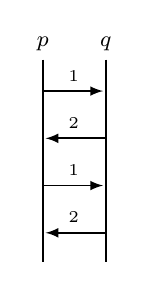
\begin{tikzpicture}[>=stealth,node distance=3.4cm,shorten >=1pt,
            every state/.style={text=black, scale =0.7}, semithick,
              font={\fontsize{8pt}{12}\selectfont}]

      \begin{scope}[shift = {(10.5,0.75)}, scale = 0.8]
        % \draw (0.5, -4) node{\textbf{(b)}};
        %MACHINES
        \draw (0,0) node{$p$} ;
        \draw (1,0) node{$q$} ;
        \draw (0,-0.25) -- (0,-3.5) ;
        \draw (1,-0.25) -- (1,-3.5);
        %MESSAGES

         \draw[>=latex,->] (0, -0.75) -- (1, -0.75) node[midway, above] {$\amessage_1$};
         \draw[>=latex,->] (1, -1.5) -- (0, -1.5) node[midway, above] {$\amessage_2$};
         \draw[>=latex,->] (0, -2.25) -- (1, -2.25) node[midway, above] {$\amessage_1$};
         \draw[>=latex,->] (1, -3) -- (0, -3) node[midway, above] {$\amessage_2$};


         %\draw (0.5, -3.25) node{$\cdots$};


      \end{scope}


              \end{tikzpicture}
              \captionof{figure}{MSC $\mscstronguniver$}
              \label{fig:msc_strong_univer}
            \end{center}

\end{minipage}
\end{center}


Similarly, \sS{} systems are incomparable with \eb{} ones.
$\systemweakS$ in Fig.~\ref{fig:system_weak_S} is \sS{} (and also \wks{1})
but, to get an execution from $\mscweakS$ we need to send message $\msg_5$ before $\msg_1$ and, as we see with $\msc_6$ previously, the number of iterations of $\msg_2$ becomes the bound of the channels for this execution. As it is unbounded, the system cannot be \eb{}.

\begin{center}
  \begin{minipage}[c]{8cm}
    

\begin{center}
\begin{tikzpicture}[>=stealth,node distance=3.4cm,shorten >=1pt,
    every state/.style={text=black, scale =0.6}, semithick,
      font={\fontsize{8pt}{12}\selectfont}]
      \begin{scope}[->, shift={(7,0)}]
          \node[state,initial,initial text={}] (q0)  {$\ell_p^0$};
          \node[state, right of=q0] (q1)  {$\ell_p^1$};

          \path (q0) edge [loop above] node [right]   {$\send{p}{q}{\msg_2}$}(q0);
          \path (q0) edge node [above] {$\rec{s}{p}{\msg_4}$} (q1);

          \node[rectangle, thick, draw] at (-0.7,0.6) {$A_p$};
      \end{scope}
      \begin{scope}[->, shift={(7,-1.25)}]
  	      \node[state,initial,initial text={}] (q0)  {$\ell_q^0$};
  				\node[state, right of=q0] (q1)  {$\ell_q^1$};
          \node[state, right of=q1] (q2)  {$\ell_q^2$};

          \path (q0) edge node [above] {$\send{q}{r}{\msg_1}$} (q1);
          \path (q1) edge [loop above] node [right]   {$\rec{p}{q}{\msg_2}$}(q1);
          \path (q1) edge node [above] {$\rec{s}{q}{\msg_3}$} (q2);

      		\node[rectangle, thick, draw] at (-0.7,0.6) {$A_q$};
  	  \end{scope}

      \begin{scope}[->, shift={(7,-2.5)}]
          \node[state,initial,initial text={}] (q0)  {$\ell_q^0$};
          \node[state, right of=q0] (q1)  {$\ell_q^1$};

          \path (q0) edge node [above] {$\rec{s}{r}{\msg_5}$} (q1);

          \node[rectangle, thick, draw] at (-0.7,0.6) {$A_r$};
      \end{scope}
      \begin{scope}[->, shift={(7,-3.75)}]
          \node[state,initial,initial text={}] (q0)  {$\ell_q^0$};
          \node[state, right of=q0] (q1)  {$\ell_q^1$};
          \node[state, right of=q1] (q2)  {$\ell_q^2$};
          \node[state, right of=q2] (q3)  {$\ell_q^3$};

          \path (q0) edge node [above] {$\send{s}{q}{\msg_3}$} (q1);
          \path (q1) edge node [above] {$\send{s}{p}{\msg_4}$} (q2);
          \path (q2) edge node [above] {$\send{s}{r}{\msg_5}$} (q3);

          \node[rectangle, thick, draw] at (-0.7,0.6) {$A_s$};
      \end{scope}
      \end{tikzpicture}
\captionof{figure}{System $\systemweakS$}
\label{fig:system_weak_S}
      \end{center}

\end{minipage}
\hspace*{1cm}
\begin{minipage}[c]{3.5cm}
  \begin{center}


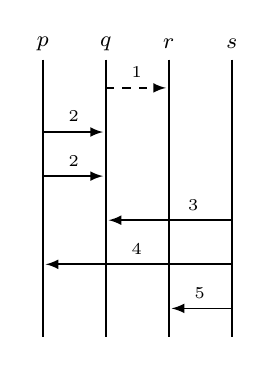
\begin{tikzpicture}[>=stealth,node distance=3.4cm,shorten >=1pt,
    every state/.style={text=black, scale =0.7}, semithick,
      font={\fontsize{8pt}{12}\selectfont}]

\begin{scope}[shift = {(8.5,0)}, scale = 0.8]

  %MACHINES
  \draw (0,0) node{$p$} ;
  \draw (1,0) node{$q$} ;
  \draw (2,0) node{$r$} ;
  \draw (3,0) node{$s$} ;
  \draw (0,-0.25) -- (0,-4.7) ;
  \draw (1,-0.25) -- (1,-4.7);
  \draw (2, -0.25) -- (2, -4.7) ;
  \draw (3, -0.25) -- (3, -4.7) ;

  %MESSAGES
  \draw[>=latex,->, dashed] (1,-0.7) -- (2, -0.7) node[midway,above]{$\amessage_1$};

  \draw[>=latex,->] (0, -1.4) -- (1, -1.4) node[midway, above] {$\amessage_2$};

  \draw[>=latex,->] (0,-2.1) -- (1,-2.1) node[midway, above] {$\amessage_2$};

  \draw[>=latex,->] (3,-2.8) -- (1,-2.8) node[pos = 0.3,above] {$\amessage_3$};

  \draw[>=latex,->] (3,-3.5) -- (0,-3.5) node[midway,above] {$\amessage_4$};

  \draw[>=latex,->] (3,-4.2) -- (2,-4.2) node[midway,above] {$\amessage_5$};

%  \draw[>=latex,->] (2,-3.25) -- (3,-3.25) node[midway,above] {$\amessage_5$};

  %\draw (0.5, -1.55) node{$\cdots$};

\end{scope}
\end{tikzpicture}
\captionof{figure}{MSC $\msc_{13}$ }
\label{fig:msc_weak_S}
\end{center}

\end{minipage}
\end{center}


$\systemWexist$ in Fig.~\ref{fig:system_W_exist} is \eb{} and \wS{}, but, again, message $\msg_5$ have to be sent before $\msg_1$, so all messages in $\mscWexist$ have to be in the same exchange. However, on process $r$, receptions of $\msg_3$ precedes send of $\msg_5$ and so this is not an exchange, and the system is not \sS{}.

%
\begin{center}
\begin{tikzpicture}[>=stealth,node distance=3.4cm,shorten >=1pt,
    every state/.style={text=black, scale =0.7}, semithick,
      font={\fontsize{8pt}{12}\selectfont}]
      \begin{scope}[->, shift={(7,0)}]
          \node[state,initial,initial text={}] (q0)  {$\ell_p^0$};
          \node[state, right of=q0] (q1)  {$\ell_p^1$};
          \node[state, right of=q1] (q2)  {$\ell_p^2$};


          \path (q0) edge node [above] {$\send{p}{q}{\msg_1}$} (q1);
          \path (q1) edge node [above]  {$\rec{q}{p}{\msg_2}$} (q2);

          \node[rectangle, thick, draw] at (-0.7,0.6) {$A_p$};
      \end{scope}
      \begin{scope}[->, shift={(7,-1.5)}]
  	      \node[state,initial,initial text={}] (q0)  {$\ell_q^0$};
  				\node[state, right of=q0] (q1)  {$\ell_q^1$};
          \node[state, right of=q1] (q2)  {$\ell_q^2$};

          \path (q0) edge [loop above] node [right]   {$\send{q}{r}{\msg_3}$}(q0);
          \path (q0) edge node [above] {$\rec{r}{q}{\msg_4}$} (q1);
          \path (q1) edge node [above] {$\rec{r}{q}{\msg_5}$} (q2);

      		\node[rectangle, thick, draw] at (-0.7,0.6) {$A_q$};
  	  \end{scope}

      \begin{scope}[->, shift={(7,-3)}]
          \node[state,initial,initial text={}] (q0)  {$\ell_q^0$};
          \node[state, right of=q0] (q1)  {$\ell_q^1$};
          \node[state, right of=q1] (q2)  {$\ell_q^2$};


          \path (q0) edge node [above] {$\send{r}{q}{\msg_4}$} (q1);
          \path (q1) edge [loop above] node [right]  {$\rec{q}{r}{\msg_3}$}(q1);
          \path (q1) edge node [above] {$\send{r}{q}{\msg_5}$} (q2);

          \node[rectangle, thick, draw] at (-0.7,0.6) {$A_q$};
      \end{scope}
      \end{tikzpicture}
\captionof{figure}{System $\systemWexist$}
\label{fig:system_W_exist}
      \end{center}


For the intersection, as with weak, a \sS{} and \eb{} systems is always \sks{k} for a $k$, by Proposition~\ref{proposition:weak_univer_uweak}. We can have for example, $\systemW$ which is \sS{}, \ub{}, \wks{1}
 but, as an exchange have to contain all messages that we have in $\msc_3$, and we can repeat $\msg_2$ as many times we want, an exchange in mailbox is no bounded, and the system is not \sks{k} for any $k$.
 We can also have $\systemWSexist$ in Fig.~\ref{fig:system_W_S_exist} which is \sS{} and \eb{} but, as one execution is always an exchange, and it can grow without limits, we cannot be neither \sks{k} nor \wks{k} for any $k$.

 %\begin{center}
\begin{tikzpicture}[>=stealth,node distance=3.4cm,shorten >=1pt,
    every state/.style={text=black, scale =0.7}, semithick,
      font={\fontsize{8pt}{12}\selectfont}]
      \begin{scope}[->, shift={(0,0)}]
          \node[state,initial,initial text={}] (q0)  {$\ell_p^0$};
          \node[state, right of=q0] (q1)  {$\ell_p^1$};

          \path (q0) edge [loop above] node [right]   {$~\send{p}{q}{\msg_1}$}(q0);
          \path (q0) edge node [below] {$\rec{q}{r}{\msg_2}$} (q1);

          \node[rectangle, thick, draw] at (-0.7,0.6) {$A_p$};
      \end{scope}
      \begin{scope}[->, shift={(0,-1.5)}]
  	      \node[state,initial,initial text={}] (q0)  {$\ell_q^0$};
  				\node[state, right of=q0] (q1)  {$\ell_q^1$};

  				\path (q0) edge node [above] {$\send{q}{r}{\msg_2}$} (q1);
          \path (q1) edge [loop right] node [right]   {$\rec{p}{q}{\msg_1}~$}(q1);


      		\node[rectangle, thick, draw] at (-0.7,0.6) {$A_q$};
  	  \end{scope}
      \end{tikzpicture}
\captionof{figure}{System $\systemWSexist$}
\label{fig:system_W_S_exist}
      \end{center}



%, and weakly synchronizable systems become incomparable with respect to existentially bounded.

%\input{diagram-mailbox-classes}

%Proposition \ref{theorem:synchro_in_exists_p2p} needs to be adapted to mailbox semantics.

%
%
% \begin{restatable}{proposition}{stronginexistsmailbox}\label{theorem:strong_in_exists_mailbox}
% 	Every \skSous{k} mailbox MSC is existentially $k$-mailbox-bounded.
% \end{restatable}
% ---------------------OLD VERSION
%
%
% By definition, \sS mailbox systems are \wS, as each MSC can be divided into exchange.
% In the same way, any \sks{k} mailbox system is \wks{k}, as each MSC can be decomposed into \kE{k}s. Note that if a system is \sks{k} with the smallest possible $k$, it can be \wks{k'} with  $k'<k$.
% However, this  is a proper inclusion. Indeed  system $\System_2$ in Fig.~\ref{fig:system_weak_exist} (when we consider the mailbox semantics)  is \wks{1} but not \sks{k} for any $k$. Messages $\msg_1$ and $\msg_3$ are constrained to be in the same \kE{k} but as we can have an unbounded number of sends and reception of $\msg_2$, the size of the \kE{k} is unbounded as well. Notice that this system is also \ekb{1}.
%
% %MSC $M_2$ in Fig.~\ref{fig:msc_weak_exist} is strongly-$3$-synchronous. But, if we add an iteration of message $\msg_2$, the corresponding MSC is strongly-$4$-synchronous. Finally, the size of the \kE{k}s is not bounded.
%
%
% Similarly, any \ukb{k} mailbox system is also \ekb{k} as all linearizations are bounded. However, the bound can  be smaller and so the system can sometimes be \ekb{k'} with $k'<k$.
% This is also a proper inclusion. Take, for instance, system $\System_5$ in Fig.~\ref{fig:system_exist}, %and an example of MSC with $M_5$ in Fig.~\ref{fig:msc_exist}
% which %, if we imagine an unbounded number of repetions of $\msg_3$,
% is \ekb{1} but not \ukb{k} for any $k$, as channel $c_r$  can be unbounded  because of the loops for  $\send{q}{r}{\msg_3}$.
% 


%\begin{figure}
  \begin{center}
      \begin{tikzpicture}[>=stealth,node distance=3.4cm,shorten >=1pt,
      every state/.style={text=black, scale =0.65}, semithick,
        font={\fontsize{8pt}{12}\selectfont}]
	% %P
  \begin{scope}[->]
     \node[state,initial,initial text={}] (q0)  {$\ell_p^0$};
     \node[state, right of=q0] (q1)  {$\ell_p^1$};
     \node[state, right of=q1] (q2) {$\ell_p^2$};

     \path (q0) edge node [above] {$\send{p}{q}{\msg_1}$} (q1);
     \path (q1) edge[bend left = 10] node [above] {$\send{p}{q}{\msg_1}$}(q2);
     \path (q2) edge[bend left = 10] node [below] {$\rec{q}{p}{\msg_2}$}(q1);

     \node[rectangle, thick, draw] at (-0.6,0.5) {$A_p$};
 \end{scope}

 \begin{scope}[->, shift={(6,0)}]
     \node[state,initial,initial text={}] (q0)  {$\ell_q^0$};
     \node[state, right of=q0] (q1)  {$\ell_q^1$};

     \path (q0) edge[bend left = 10] node [above] {$\send{q}{p}{\msg_2}$} (q1);
      \path (q1) edge[bend left = 10] node [below] {$\rec{p}{q}{\msg_1}$} (q0);
      \path (q0) edge [loop below] node [below]   {$~\send{q}{r}{\msg_3}$}(q0);
      \path (q1) edge [loop below] node [below]   {$~\send{q}{r}{\msg_3}$}(q1);


     \node[rectangle, thick, draw] at (-0.6,0.5) {$A_q$};
 \end{scope}

\begin{scope}[->, shift ={(11, 0)}]
   \node[state,initial,initial text={}] (q0)  {$\ell_r^0$};
   \path (q0) edge [loop below] node [below]   {$~\rec{q}{r}{\msg_3}$}(q0);
   \node[rectangle, thick, draw] at (-0.6,0.5) {$A_r$};

\end{scope}


		% \begin{scope}[shift = {(7.5,0.5)}, scale = 0.8]
    %   \draw (1.25, -4.75) node{\textbf{(b existe plus haut)}};
    %   \draw (-8, -4.75) node{\textbf{(a)}};
    %
		% 	%MACHINES
		% 	\draw (0,0) node{$p$} ;
		% 	\draw (1.25,0) node{$q$} ;
    %   \draw (2.5,0) node{$r$} ;
		% 	\draw (2.5, -0.25) -- (2.5, -3.75) ;
		% 	\draw (0,-0.25) -- (0,-3.75) ;
		% 	\draw (1.25,-0.25) -- (1.25,-3.75);
		% 	%MESSAGES
    %
    %   \draw[>=latex,->] (0, -0.5) -- (1.25, -1.25) node[pos=0.4, sloped, above] {$\amessage_1$};
    %   \draw[>=latex,->] (0, -1.5) -- (1.25, -2.25) node[pos=0.5, sloped, above] {$\amessage_1$};
    %   \draw[>=latex,->] (0, -2.5) -- (1.25, -3.25) node[pos=0.65, sloped, above] {$\amessage_1$};
    %
    %   \draw[>=latex,->] (1.25, -0.75) -- (0, -2) node[pos=0.5, sloped, above] {$\amessage_2$};
    %   \draw[>=latex,->] (1.25, -1.75) -- (0, -3) node[pos=0.5, sloped, above] {$\amessage_2$};
    %
    %   \draw[>=latex,->] (1.25, -1) -- (2.5, -1) node[midway, above] {$\amessage_3$};
    %   \draw[>=latex,->] (1.25, -1.5) -- (2.5, -1.5) node[midway, above] {$\amessage_3$};
    %   \draw[>=latex,->] (1.25, -2.5) -- (2.5, -2.5) node[midway, above] {$\amessage_3$};
    %
    %   \draw (0.6, -3.35) node{$\cdots$};
    %   \draw (1.9, -3.35) node{$\cdots$};
    %
    %
		% \end{scope}
\end{tikzpicture}
\captionof{figure}{System $\systemexist$}
\label{fig:system_exist}

\end{center}

%\end{figure}

%
%
%
% The class of weakly synchronizable systems is incomparable with the class of existentially bounded. Indeed,   system $\System_6$ below is \wks{1} but  not \ekb{k} for any $k$. As exemplified in Fig. \ref{fig:msc_weak}, MSCs can be  divided into \kE{1}s.  But when we linearize them, $\msg_4$ has to be sent before $\msg_1$ and  all messages $\msg_2$ have to be sent before  $\msg_4$. The reception of  $\msg_2$ can start only when $\msg_1$ has been sent. Hence  we can have an unbounded number of $\msg_2$ and therefore the size of channel $c_q$ is also unbounded.
% \begin{center}
%  \noindent
%  \begin{minipage}[b]{7.75cm}
% 
  \begin{center}

  \begin{tikzpicture}[>=stealth,node distance=3.4cm,shorten >=1pt,
      every state/.style={text=black, scale =0.65}, semithick,
        font={\fontsize{8pt}{12}\selectfont}]

        \begin{scope}[-> ]
            \node[state,initial,initial text={}] (q0)  {$\ell_p^0$};
            \node[state, right of=q0] (q1)  {$\ell_p^1$};
            \node[state, right of=q1] (q2) {$\ell_p^2$};

            \path (q0) edge node [above] {$\send{p}{q}{\msg_2}$} (q1);
            \path (q1) edge [loop above] node [right]   {$~\send{p}{q}{\msg_2}$}(q1);
            \path (q1) edge node [above] {$\send{p}{s}{\msg_3}$}(q2);
            \node[rectangle, thick, draw] at (-0.6,0.6) {$A_p$};
        \end{scope}


      \begin{scope}[->,  shift={(0,-1.1)}]
          \node[state,initial,initial text={}] (q0)  {$\ell_q^0$};
          \node[state, right of=q0] (q1)  {$\ell_q^1$};
          \node[state, right of=q1] (q2) {$\ell_q^2$};

          \path (q0) edge node [above] {$\send{q}{r}{\msg_1}$} (q1);
          \path (q1) edge node [above] {$\rec{p}{q}{\msg_2}$}(q2);
          \path (q2) edge [loop above] node [right]   {$~\rec{p}{q}{\msg_2}$}(q2);

          \node[rectangle, thick, draw] at (-0.6,0.6) {$A_q$};
      \end{scope}



      \begin{scope}[->, shift={(0,-2.2)} ]
          \node[state,initial,initial text={}] (q0)  {$\ell_r^0$};
          \node[state, right of=q0] (q1)  {$\ell_r^1$};

          \path (q0) edge node [above] {$\rec{s}{r}{\msg_4}$} (q1);

          \node[rectangle, thick, draw] at (-0.6,0.6) {$A_r$};
        %\node at (1, -1.5) {\textbf{(a)}};

      \end{scope}
      \begin{scope}[->, shift ={(0, -3.3)}]
         \node[state,initial,initial text={}] (q0)  {$\ell_s^0$};
         \node[state, right of=q0] (q1)  {$\ell_s^1$};
         \node[state, right of=q1] (q2) {$\ell_s^2$};

         \path (q0) edge node [above] {$\rec{p}{s}{\msg_3}$} (q1);
         \path (q1) edge node [above] {$\send{s}{r}{\msg_4}$} (q2);

         \node[rectangle, thick, draw] at (-0.6,0.6) {$A_s$};

      \end{scope}
      % \begin{scope}[shift = {(8.5,0)}, scale = 0.8]
      %   \draw (1.5, -4.75) node{\textbf{(b)}};
      %   \draw (-9.5, -4.75) node{\textbf{(a)}};
      %
      %   %MACHINES
      %   \draw (0,0) node{$p$} ;
    	% 	\draw (1,0) node{$q$} ;
    	% 	\draw (2,0) node{$r$} ;
      %   \draw (3,0) node{$s$} ;
    	% 	\draw (0,-0.25) -- (0,-3.75) ;
    	% 	\draw (1,-0.25) -- (1,-3.75);
    	% 	\draw (2, -0.25) -- (2, -3.75) ;
      %   \draw (3, -0.25) -- (3, -3.75) ;
      %
    	% 	%MESSAGES
    	% 	\draw[>=latex,->, dashed] (1,-0.7) -- (2, -0.7) node[midway,above]{$\amessage_1$};
      %
    	% 	\draw[>=latex,->] (0, -1.35) -- (1, -1.35) node[midway, above] {$\amessage_2$};
      %
    	% 	\draw[>=latex,->] (0,-2.1) -- (1,-2.1) node[midway, above] {$\amessage_2$};
      %
    	% 	\draw[>=latex,->] (0,-2.75) -- (3,-2.75) node[midway,above] {$\amessage_3$};
      %
      %   \draw[>=latex,->] (3,-3.4) -- (2,-3.4) node[midway,above] {$\amessage_4$};
      %
      % %  \draw[>=latex,->] (2,-3.25) -- (3,-3.25) node[midway,above] {$\amessage_5$};
      %
      %   \draw (0.5, -1.55) node{$\cdots$};
      %
      % \end{scope}


  \end{tikzpicture}
  \captionof{figure}{System $\systemweak$ }
  \label{fig:system_weak}

\end{center}

% \end{minipage}
%  \begin{minipage}[b]{4cm}
%    \begin{center}


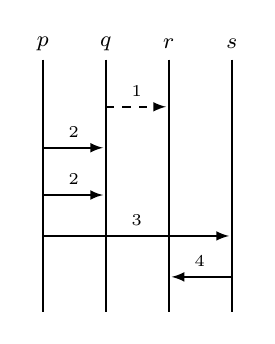
\begin{tikzpicture}[>=stealth,node distance=3.4cm,shorten >=1pt,
    every state/.style={text=black, scale =0.7}, semithick,
      font={\fontsize{8pt}{12}\selectfont}]

\begin{scope}[shift = {(8.5,0)}, scale = 0.8]

  %MACHINES
  \draw (0,0.3) node{$p$} ;
  \draw (1,0.3) node{$q$} ;
  \draw (2,0.3) node{$r$} ;
  \draw (3,0.3) node{$s$} ;
  \draw (0,0.05) -- (0,-4) ;
  \draw (1,0.05) -- (1,-4);
  \draw (2, 0.05) -- (2, -4) ;
  \draw (3, 0.05) -- (3, -4) ;

  %MESSAGES
  \draw[>=latex,->, dashed] (1,-0.7) -- (2, -0.7) node[midway,above]{$\amessage_1$};

  \draw[>=latex,->] (0, -1.35) -- (1, -1.35) node[midway, above] {$\amessage_2$};

  \draw[>=latex,->] (0,-2.1) -- (1,-2.1) node[midway, above] {$\amessage_2$};

  \draw[>=latex,->] (0,-2.75) -- (3,-2.75) node[midway,above] {$\amessage_3$};

  \draw[>=latex,->] (3,-3.4) -- (2,-3.4) node[midway,above] {$\amessage_4$};

%  \draw[>=latex,->] (2,-3.25) -- (3,-3.25) node[midway,above] {$\amessage_5$};

  %\draw (0.5, -1.55) node{$\cdots$};

\end{scope}
\end{tikzpicture}
\captionof{figure}{MSC $\mscweak$ }
\label{fig:msc_weak}
\end{center}

%  \end{minipage}
%
%  \end{center}
%
%
% As for \pp semantics,  universally bounded systems are incomparable with the weakly synchronizable ones.
% There are systems in both classes like $\System_1$ in Fig.~\ref{fig:system_weak_univer} which is \ukb{1} and \wks{1}. Some systems are \ukb{k} but not \wks{k'} for any $k'$ as $\System_3$ in Fig.~\ref{fig:system_univer}:  notice that a system, with two machines only, behaves in the same way in the \pp and mailbox semantics, thus the discussion presented above works for the mailbox semantics as well.
% %The MSC $M_3$ in Fig.~\ref{fig:system_univer} shows a possible behaviour of this system which cannot be divided into \kE{k}s, all messages of the execution have to be in the same \kE{k} but we cannot put all sends before all receptions. On the other hand, we see that each executions is at most $2$-bounded, as we need to read to send an other message.
% System $\System_4$ below is \wks{1} (and \sks{1}) but not \ukb{k} for any $k$. Indeed, channel $c_p$ can be filled by an unbounded number of messages $\msg_1$.
% \begin{center}

  \begin{tikzpicture}[>=stealth,node distance=3.4cm,shorten >=1pt,
      every state/.style={text=black, scale =0.65}, semithick,
        font={\fontsize{8pt}{12}\selectfont}]


      \begin{scope}[->, shift={(0,0)}]
          \node[state,initial,initial text={}] (q0)  {$\ell_p^0$};
           \path (q0) edge [loop right] node [right]   {$~\send{p}{q}{\msg_1}$}(q0);
          \node[rectangle, thick, draw] at (-0.6,0.6) {$A_p$};
      \end{scope}

     \begin{scope}[->, shift ={(4, 0)}]
        \node[state,initial,initial text={}] (q0)  {$\ell_q^0$};
        \path (q0) edge [loop right] node [right]   {$~\rec{p}{q}{\msg_1}$}(q0);
        \node[rectangle, thick, draw] at (-0.6,0.6) {$A_q$};
     \end{scope}
\end{tikzpicture}
\captionof{figure}{System $\systemstrongexist$}
\label{fig:system_strong_exist}
\end{center}

% The class of universally bounded systems is also incomparable with the classes of strongly synchronizable systems.
% As for \pp, system $\System_3$ is not \sks{k}  for any $k$ but  it is  \ukb{3}.  Still the properties are not incompatible,  for instance, system $\System_7$ below  is both \ukb{1} and \sks{1}.
% \begin{center}
%  \noindent
%  \begin{minipage}[b]{5cm}
% 
\begin{center}
\begin{tikzpicture}[>=stealth,node distance=3.4cm,shorten >=1pt,
    every state/.style={text=black, scale =0.7}, semithick,
      font={\fontsize{8pt}{12}\selectfont}]
      \begin{scope}[->, shift={(0,0)}]
          \node[state,initial,initial text={}] (q0)  {$\ell_p^0$};
          \node[state, right of=q0] (q1)  {$\ell_p^1$};

          \path (q0) edge[bend left = 10] node [above] {$\send{p}{q}{\msg_1}$} (q1);
          \path (q1) edge[bend left = 10] node [below] {$\rec{q}{r}{\msg_2}$} (q0);

          \node[rectangle, thick, draw] at (-0.7,0.6) {$A_p$};
      \end{scope}
      \begin{scope}[->, shift={(4,0)}]
  	      \node[state,initial,initial text={}] (q0)  {$\ell_q^0$};
  				\node[state, right of=q0] (q1)  {$\ell_q^1$};

  				\path (q0) edge[bend left = 10] node [above] {$\rec{p}{q}{\msg_1}$} (q1);
          \path (q1) edge[bend left = 10] node [below] {$\send{q}{p}{\msg_2}$} (q0);

      		\node[rectangle, thick, draw] at (-0.7,0.6) {$A_q$};
  	  \end{scope}
      \end{tikzpicture}
\captionof{figure}{System $\systemstronguniver$}
\label{fig:system_strong_univer}
      \end{center}

%  \end{minipage}
%  \begin{minipage}[b]{5cm}
% 



      \begin{center}
        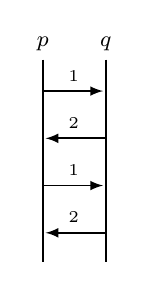
\begin{tikzpicture}[>=stealth,node distance=3.4cm,shorten >=1pt,
            every state/.style={text=black, scale =0.7}, semithick,
              font={\fontsize{8pt}{12}\selectfont}]

      \begin{scope}[shift = {(10.5,0.75)}, scale = 0.8]
        % \draw (0.5, -4) node{\textbf{(b)}};
        %MACHINES
        \draw (0,0) node{$p$} ;
        \draw (1,0) node{$q$} ;
        \draw (0,-0.25) -- (0,-3.5) ;
        \draw (1,-0.25) -- (1,-3.5);
        %MESSAGES

         \draw[>=latex,->] (0, -0.75) -- (1, -0.75) node[midway, above] {$\amessage_1$};
         \draw[>=latex,->] (1, -1.5) -- (0, -1.5) node[midway, above] {$\amessage_2$};
         \draw[>=latex,->] (0, -2.25) -- (1, -2.25) node[midway, above] {$\amessage_1$};
         \draw[>=latex,->] (1, -3) -- (0, -3) node[midway, above] {$\amessage_2$};


         %\draw (0.5, -3.25) node{$\cdots$};


      \end{scope}


              \end{tikzpicture}
              \captionof{figure}{MSC $\mscstronguniver$}
              \label{fig:msc_strong_univer}
            \end{center}

%  \end{minipage}
%  \end{center}
